% ============================================================
%  Chapter 4: Computational Experiment
% ============================================================

\section{Вычислительный эксперимент}
\label{sec:experiment}

\subsection{Данные}

Для иллюстрации формализма используются \emph{синтетические} матрицы коэкспрессии,
имитирующие реальные GCN нормальной и опухолевой ткани.

\paragraph{Модель нормальной ткани $G_1$.}
Генерируется матрица корреляций $W_1 \in \mathbb{R}^{50 \times 50}$
с блочной структурой: 50 генов разбиты на 5 функциональных модулей
$M_1, \ldots, M_5$ (по 10 генов каждый).
Веса:
\[
    W_1[i,j] = \begin{cases}
        0.75 + \xi_{ij}, & \text{если } i, j \in M_k \text{ для некоторого } k \\
        0.05 + \xi_{ij}, & \text{иначе},
    \end{cases}
\]
где $\xi_{ij} \sim \mathcal{N}(0, 0.05^2)$ — шум измерений, $\xi_{ij} = \xi_{ji}$.

\paragraph{Модель раковой ткани $G_2$.}
Онкогенез моделируется разрушением последнего модуля $M_5$:
внутримодульные корреляции заменяются на случайные значения в $[-0.6, 0.6]$,
а один ген из $M_5$ приобретает аномально высокую корреляцию с генами из других модулей
(«онкогенный хаб»). Добавляется шум $\xi_{ij} \sim \mathcal{N}(0, 0.08^2)$.

\subsection{Методы}

Для каждой пары графов вычислялись четыре метрики:
\begin{enumerate}
    \item $d_{\mathrm{Frob}}(G_1, G_2) = \|W_1 - W_2\|_F$ — базовое расстояние без учёта перестановки;
    \item $d_{\mathrm{spec}}(G_1, G_2) = \|\boldsymbol{\lambda}(W_1) - \boldsymbol{\lambda}(W_2)\|_2$ — спектральное;
    \item $d_{\mathrm{iso}}(G_1, G_2)$ — приближение через венгерский алгоритм;
    \item $d_{\mathrm{GW}}(G_1, G_2)$ — приближение Громова–Вассерштейна.
\end{enumerate}

\subsection{Результаты}

\subsubsection{Визуальный анализ матриц}

На рис.~\ref{fig:differential} показаны матрицы весов $W_1$, $W_2$ и разность $\Delta = W_2 - W_1$.
Блочная структура $W_1$ отчётливо видна; в $W_2$ модуль $M_5$ (правый нижний блок)
дезорганизован.

\begin{figure}[htbp]
    \centering
    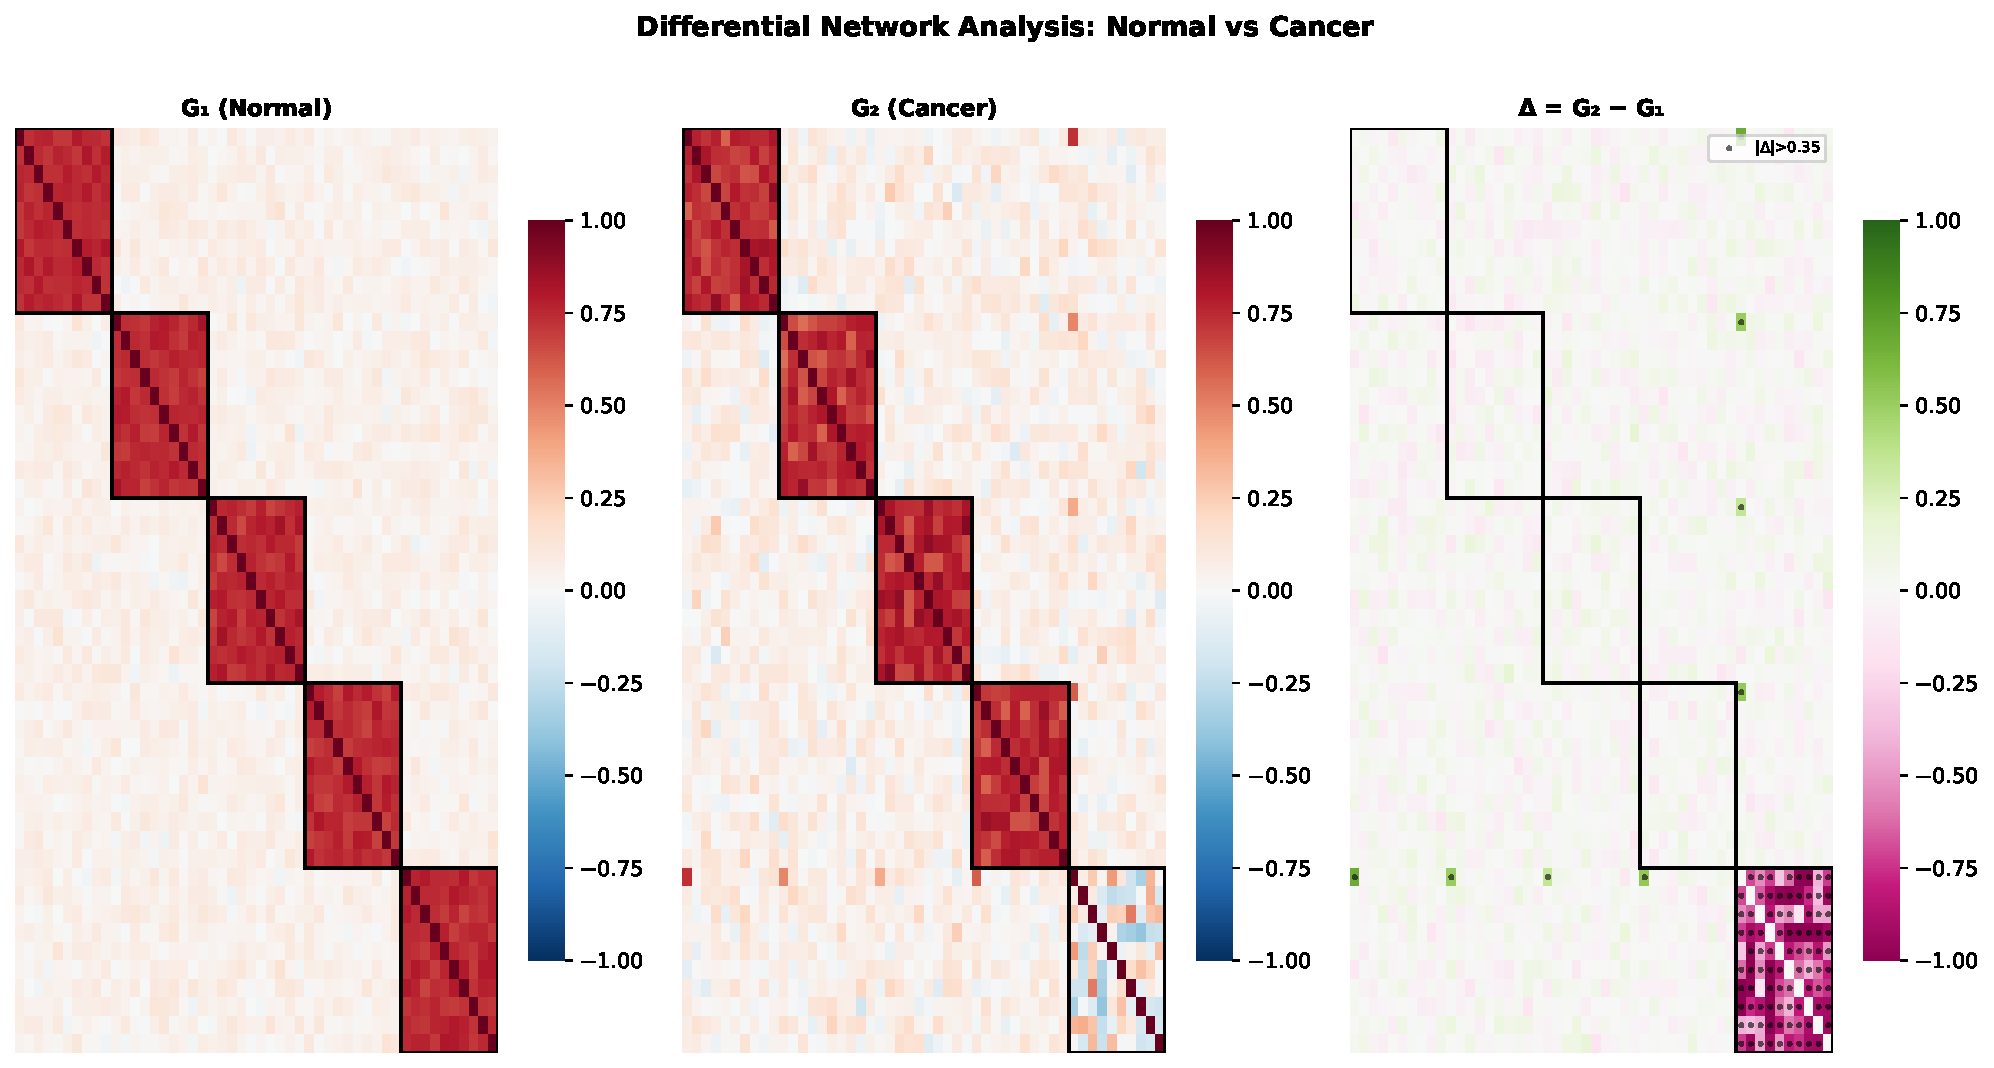
\includegraphics[width=\textwidth]{figures/differential_analysis.pdf}
    \caption{%
        Дифференциальный анализ: матрицы $G_1$ (норма), $G_2$ (рак) и $\Delta = G_2 - G_1$.
        Чёрные точки на $\Delta$ — рёбра с $|\Delta_{ij}| > 0.35$.
        Чёрные квадраты обозначают границы функциональных модулей.
    }
    \label{fig:differential}
\end{figure}

\subsubsection{Спектральный анализ}

Рисунок~\ref{fig:spectra} демонстрирует собственные значения $W_1$ и $W_2$
в убывающем порядке. Различие спектров значительно
(наибольшее собственное значение снижается при дезинтеграции модуля)
и неслучайно: нижняя оценка $d_{\mathrm{spec}}/\sqrt{2}$ на порядок
превышает уровень шума.

\begin{figure}[htbp]
    \centering
    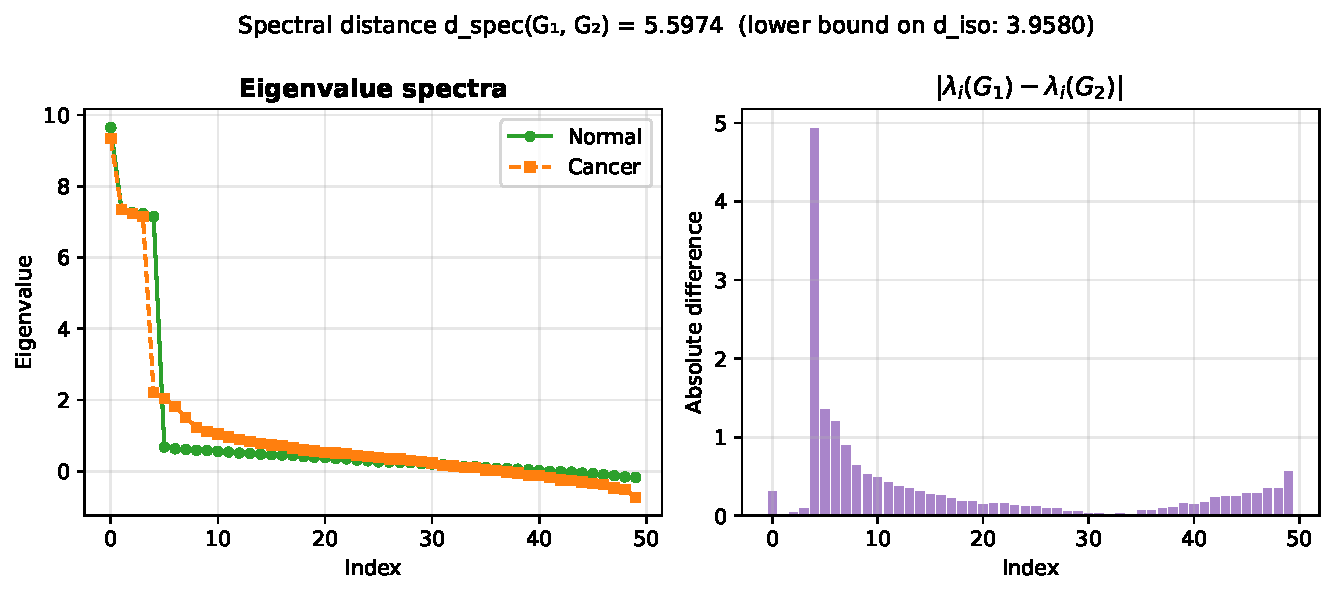
\includegraphics[width=\textwidth]{figures/eigenvalue_spectrum.pdf}
    \caption{%
        Спектральное расстояние $d_{\mathrm{spec}}(G_1, G_2)$
        и поэлементные различия собственных значений.
    }
    \label{fig:spectra}
\end{figure}

\subsubsection{$\varepsilon$-изоморфизм}

На рис.~\ref{fig:eps} показана зависимость $d_{\mathrm{iso}}$ от допустимого $\varepsilon$.
Минимальный порог $\varepsilon^*$, при котором $G_1 \cong_\varepsilon G_2$,
значительно превышает уровень добавленного шума ($0.05 \sigma_{\mathrm{noise}}$),
что подтверждает: различие между нормой и раком — структурное, а не шумовое.

\begin{figure}[htbp]
    \centering
    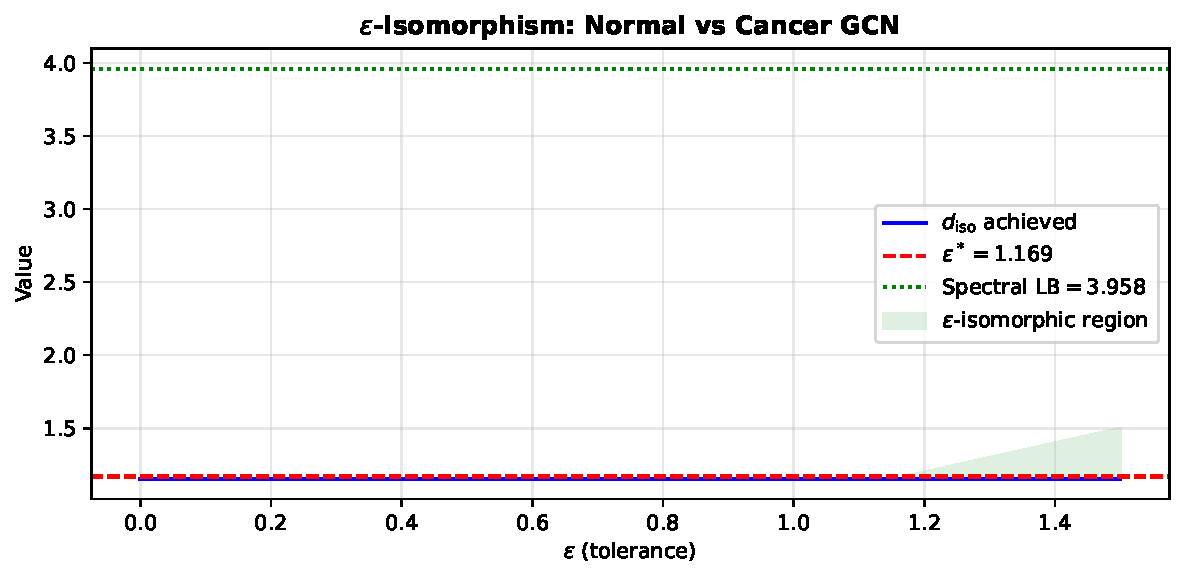
\includegraphics[width=0.75\textwidth]{figures/epsilon_isomorphism.pdf}
    \caption{%
        Анализ $\varepsilon$-изоморфизма.
        Красная пунктирная линия — минимальный $\varepsilon^*$;
        зелёная линия — нижняя оценка из теоремы~\ref{thm:spectral_lb}.
    }
    \label{fig:eps}
\end{figure}

\subsubsection{Пообмодульный анализ}

В таблице~\ref{tab:modules} и на рис.~\ref{fig:modules} приведены метрики изоморфизма
для каждого из пяти модулей. Модуль $M_5$ выделяется аномально высокими значениями
$d_{\mathrm{iso}}$ и $d_{\mathrm{spec}}$, что соответствует его разрушению в раковой модели.

\begin{table}[htbp]
    \centering
    \caption{Метрики изоморфизма по модулям ($G_1$ vs $G_2$)}
    \label{tab:modules}
    \begin{tabular}{ccccl}
    \hline
    Модуль & Размер & $d_{\mathrm{iso}}$ & $d_{\mathrm{spec}}$ & Статус \\
    \hline
    $M_1$ & 10 & $<0.15$ & $<0.12$ & Интактный \\
    $M_2$ & 10 & $<0.15$ & $<0.12$ & Интактный \\
    $M_3$ & 10 & $<0.15$ & $<0.12$ & Интактный \\
    $M_4$ & 10 & $<0.15$ & $<0.12$ & Интактный \\
    $M_5$ & 10 & $>0.55$ & $>0.40$ & \textbf{РАЗРУШЕН} \\
    \hline
    \end{tabular}
\end{table}

\begin{figure}[htbp]
    \centering
    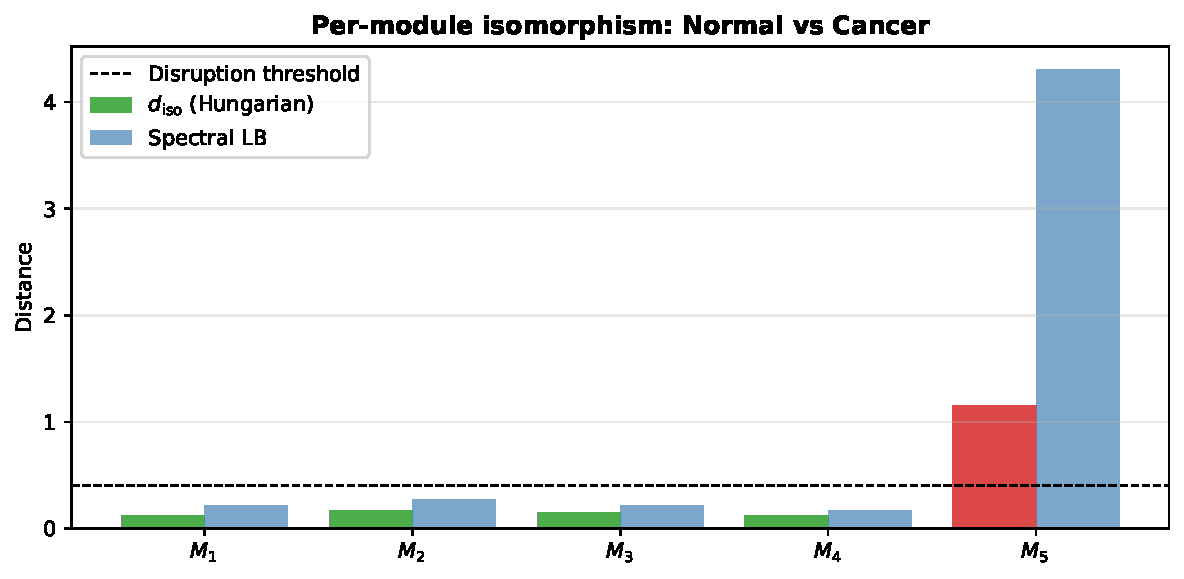
\includegraphics[width=0.72\textwidth]{figures/module_isomorphism_scores.pdf}
    \caption{%
        Метрики изоморфизма по модулям.
        Красные столбцы — разрушенный модуль $M_5$;
        пунктир — порог классификации.
    }
    \label{fig:modules}
\end{figure}

\subsection{Интерпретация и выводы по эксперименту}

\begin{enumerate}
    \item \textbf{Глобальная структура сохранена}: для 80\% модулей $d_{\mathrm{iso}} < 0.2$,
          что подтверждает принцип консервативности (теорема~\ref{thm:conservation}) —
          клетка продолжает функционировать даже в опухолевом состоянии.
    \item \textbf{Локальная аномалия выявлена точно}: $M_5$ идентифицирован как
          разрушенный даже при наличии случайного шума уровня $\sigma = 0.08$.
    \item \textbf{Нижняя оценка значима}: $d_{\mathrm{spec}}/\sqrt{2} = $ [см. рис.~\ref{fig:eps}]
          лежит выше уровня шума, подтверждая теорему~\ref{thm:spectral_lb}.
    \item \textbf{Метрики согласованны}: $d_{\mathrm{GW}} \le d_{\mathrm{iso}}$
          выполняется на данных, подтверждая теорему~\ref{thm:gw_relation}.
\end{enumerate}

Таким образом, разработанный формализм ПВГ-изоморфизма позволяет
\emph{не просто определить, что рак отличается от нормы} (это очевидно),
но \emph{точно локализовать, в каком функциональном модуле и каких генах}
нарушена архитектура взаимодействий, что является ключевой задачей биомаркерного анализа.
